\chapter{Pushing III: Real-robot application}

At this point, we know that a pushing task can be learned, at least with some
simplifications and using the Deep Deterministic Policy Gradient (DDPG)
approach. Preliminary experiments were done in simulation, where noise was
added equivalent to the noise expected from the real robotic system, but failed
to converge to any decent policy. Also, all the previous experiments in
simulation were harder than anticipated and consumed several weeks before
finally solving the problem. Instead of further investigating training on the
real robotic systems from this point on, the policy trained in simulation is
briefly evaluated on the real robotic system before continuing with
investigating pose estimation methods.

\section{Method}

To estimate the pose of the cube, a LIDAR was used by placing it in front of
the robot arm (figure \ref{fig:eef-frame}). The cube to push was a red wooden
cube with all sides measuring $4$ cm. One of these sides can be found from the
LIDAR-measurements by plotting the points onto a matrix/image and using the
Hough transform \cite{duda1972use}, see section \ref{sec:method_hough}. For the following experiments, only the
position of the cube was kept, ignoring the rotation. Conversion of the found
position of the cube to robot-frame was done using a least-squares approach
after randomly placing the cube at several positions known from the
forward-kinematics of the arm.

\begin{figure}[h!]
    \centering
    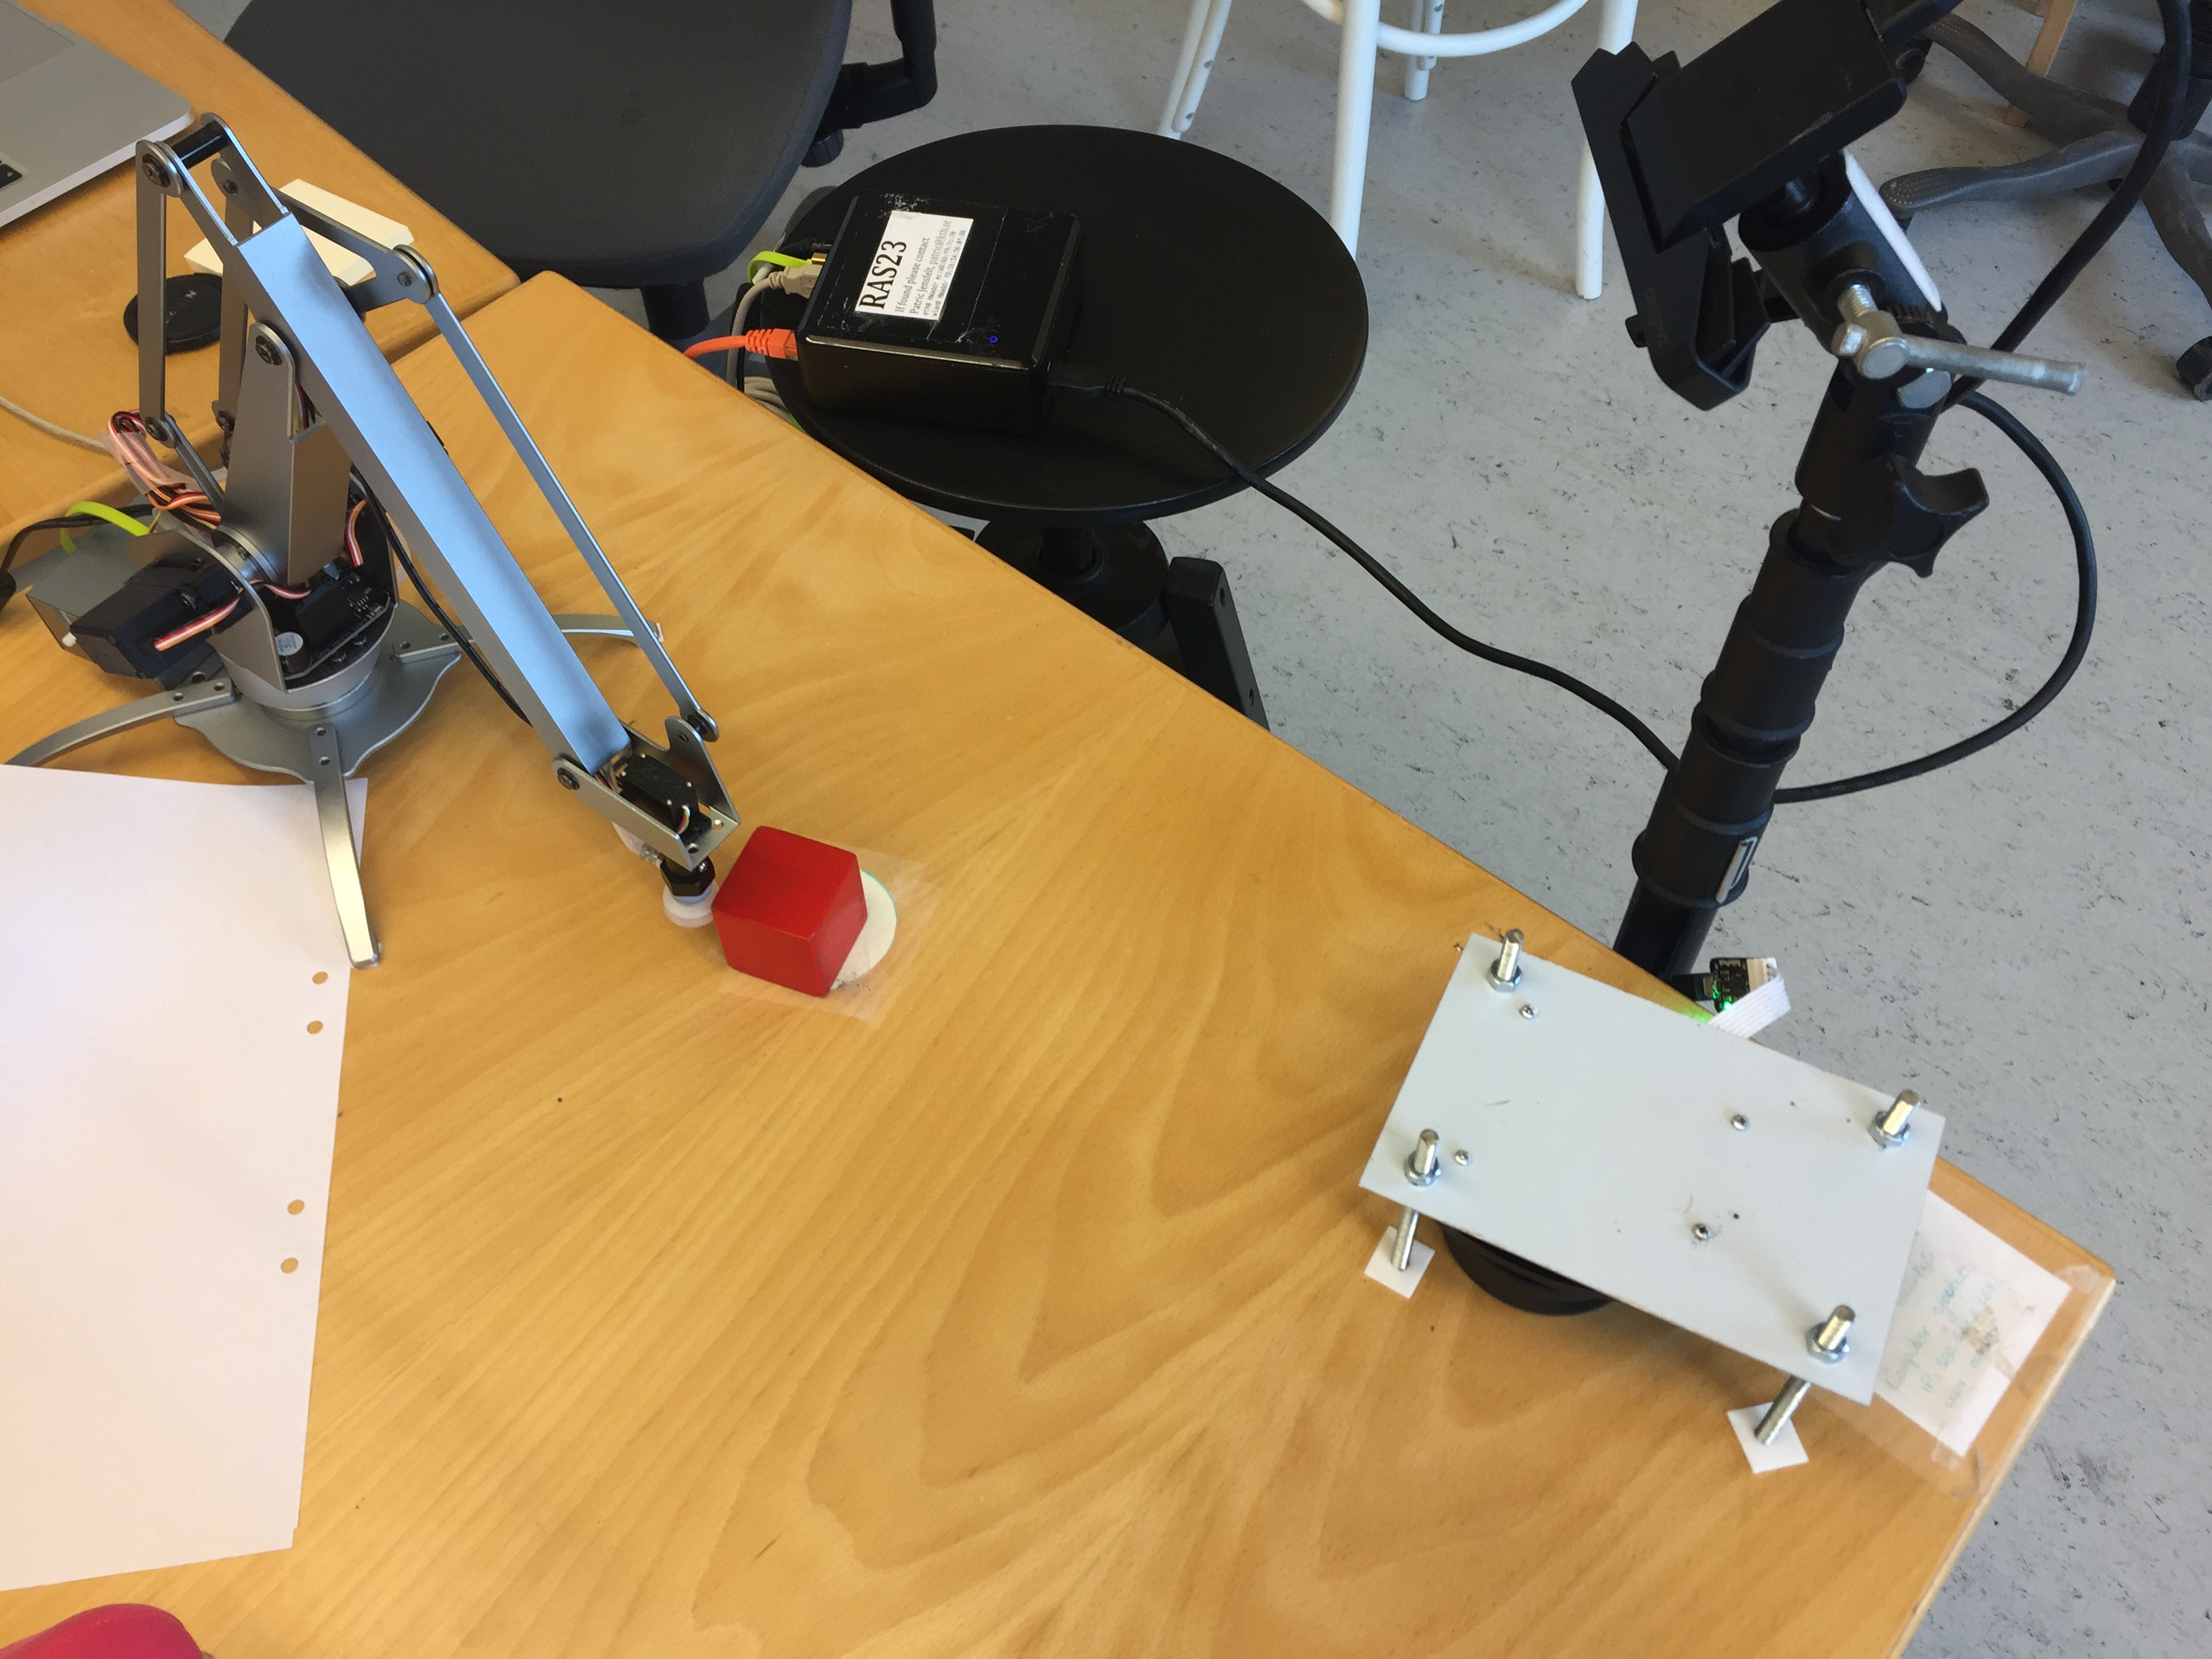
\includegraphics[width=0.48 \textwidth]{res/camera_placement_fixed.jpg}

    \caption{LIDAR seen on the right side in the picture measuring positions of
    the cube. The camera is not used in this experiment.}

    \label{fig:eef-frame}
    
\end{figure}

\section{Results}

The policy trained in simulation successfully pushes the cube towards a goal
set in the center of the workspace, video of this can be seen here:
\url{https://youtu.be/82XNDBPbJH0}. Sometimes the policy fails to push the cube
further due to small action commands not affecting the robot, and due to
differences in the shapes of the simulation object (circle) and the cube.
Adding a small noise term alleviated these problems and was used in the linked
video.
